\begin{tikzpicture}[scale=.2, anchor=west]
\node[draw opacity=0, fill opacity=0, anchor=south west] (dummyL) at (-3, -15){};
\node[draw=black, rectangle split, anchor=south west, rectangle split parts=3] (sn0x8eb820) at ([xshift=2cm]dummyL){
\begin{tikzpicture}[scale=.2]
\node[circle, scale=0.75, fill] (tid0) at (3,0){};
\node[circle, scale=0.75, fill] (tid1) at (2.25,1.5){};
\node[circle, scale=0.75, fill] (tid3) at (1.5,3){};
\node[circle, scale=0.75, fill, red] (tid6) at (0.75,4.5){};
\node[circle, scale=0.75, fill, red] (tid7) at (2.25,4.5){};
\draw[](tid3) -- (tid6);
\draw[](tid3) -- (tid7);
\node[circle, scale=0.75, fill] (tid4) at (3.75,3){};
\draw[](tid1) -- (tid3);
\draw[](tid1) -- (tid4);
\node[circle, scale=0.75, fill] (tid2) at (5.25,1.5){};
\node[circle, scale=0.75, fill, red] (tid5) at (5.25,3){};
\draw[](tid2) -- (tid5);
\draw[](tid0) -- (tid1);
\draw[](tid0) -- (tid2);

\end{tikzpicture}
\nodepart{two}
\footnotesize{4.99537}
\nodepart{three}
\footnotesize{$33\:67$}
};
\node[draw opacity=0, fill opacity=0, anchor=south west] (dummyL) at (-6, -30){};
\node[draw=black, rectangle split, anchor=south west, rectangle split parts=3] (sn0x8ee960) at ([xshift=2cm]dummyL){
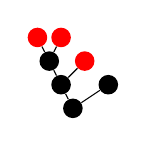
\begin{tikzpicture}[scale=.2]
\node[circle, scale=0.75, fill] (tid0) at (3,0){};
\node[circle, scale=0.75, fill] (tid1) at (2.25,1.5){};
\node[circle, scale=0.75, fill] (tid3) at (1.5,3){};
\node[circle, scale=0.75, fill, red] (tid5) at (0.75,4.5){};
\node[circle, scale=0.75, fill, red] (tid6) at (2.25,4.5){};
\draw[](tid3) -- (tid5);
\draw[](tid3) -- (tid6);
\node[circle, scale=0.75, fill, red] (tid4) at (3.75,3){};
\draw[](tid1) -- (tid3);
\draw[](tid1) -- (tid4);
\node[circle, scale=0.75, fill] (tid2) at (5.25,1.5){};
\draw[](tid0) -- (tid1);
\draw[](tid0) -- (tid2);

\end{tikzpicture}
\nodepart{two}
\footnotesize{4.75926}
\nodepart{three}
\footnotesize{$33\:67$}
};
\node[draw opacity=0, fill opacity=0, anchor=south west] (dummyL) at (-6, -30){};
\node[draw=black, rectangle split, anchor=south west, rectangle split parts=3] (sn0x8ee260) at ([xshift=2cm]sn0x8ee960.south east){
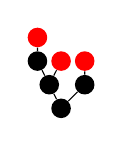
\begin{tikzpicture}[scale=.2]
\node[circle, scale=0.75, fill] (tid0) at (2.25,0){};
\node[circle, scale=0.75, fill] (tid1) at (1.5,1.5){};
\node[circle, scale=0.75, fill] (tid3) at (0.75,3){};
\node[circle, scale=0.75, fill, red] (tid6) at (0.75,4.5){};
\draw[](tid3) -- (tid6);
\node[circle, scale=0.75, fill, red] (tid4) at (2.25,3){};
\draw[](tid1) -- (tid3);
\draw[](tid1) -- (tid4);
\node[circle, scale=0.75, fill] (tid2) at (3.75,1.5){};
\node[circle, scale=0.75, fill, red] (tid5) at (3.75,3){};
\draw[](tid2) -- (tid5);
\draw[](tid0) -- (tid1);
\draw[](tid0) -- (tid2);

\end{tikzpicture}
\nodepart{two}
\footnotesize{4.61343}
\nodepart{three}
\footnotesize{$33\:33\:33$}
};
\node[draw opacity=0, fill opacity=0, anchor=south west] (dummyL) at (-12, -45){};
\node[draw=black, rectangle split, anchor=south west, rectangle split parts=3] (sn0x8ef400) at ([xshift=2cm]dummyL){
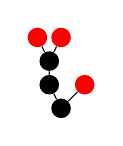
\begin{tikzpicture}[scale=.2]
\node[circle, scale=0.75, fill] (tid0) at (2.25,0){};
\node[circle, scale=0.75, fill] (tid1) at (1.5,1.5){};
\node[circle, scale=0.75, fill] (tid3) at (1.5,3){};
\node[circle, scale=0.75, fill, red] (tid4) at (0.75,4.5){};
\node[circle, scale=0.75, fill, red] (tid5) at (2.25,4.5){};
\draw[](tid3) -- (tid4);
\draw[](tid3) -- (tid5);
\draw[](tid1) -- (tid3);
\node[circle, scale=0.75, fill, red] (tid2) at (3.75,1.5){};
\draw[](tid0) -- (tid1);
\draw[](tid0) -- (tid2);

\end{tikzpicture}
\nodepart{two}
\footnotesize{4.58333}
\nodepart{three}
\footnotesize{$33\:67$}
};
\node[draw opacity=0, fill opacity=0, anchor=south west] (dummyL) at (-12, -45){};
\node[draw=black, rectangle split, anchor=south west, rectangle split parts=3] (sn0x8ef140) at ([xshift=2cm]sn0x8ef400.south east){
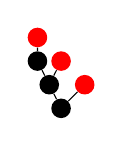
\begin{tikzpicture}[scale=.2]
\node[circle, scale=0.75, fill] (tid0) at (2.25,0){};
\node[circle, scale=0.75, fill] (tid1) at (1.5,1.5){};
\node[circle, scale=0.75, fill] (tid3) at (0.75,3){};
\node[circle, scale=0.75, fill, red] (tid5) at (0.75,4.5){};
\draw[](tid3) -- (tid5);
\node[circle, scale=0.75, fill, red] (tid4) at (2.25,3){};
\draw[](tid1) -- (tid3);
\draw[](tid1) -- (tid4);
\node[circle, scale=0.75, fill, red] (tid2) at (3.75,1.5){};
\draw[](tid0) -- (tid1);
\draw[](tid0) -- (tid2);

\end{tikzpicture}
\nodepart{two}
\footnotesize{4.34722}
\nodepart{three}
\footnotesize{$33\:33\:33$}
};
\node[draw opacity=0, fill opacity=0, anchor=south west] (dummyL) at (-12, -45){};
\node[draw=black, rectangle split, anchor=south west, rectangle split parts=3] (sn0x8f19a0) at ([xshift=2cm]sn0x8ef140.south east){
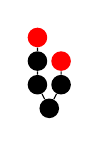
\begin{tikzpicture}[scale=.2]
\node[circle, scale=0.75, fill] (tid0) at (1.5,0){};
\node[circle, scale=0.75, fill] (tid1) at (0.75,1.5){};
\node[circle, scale=0.75, fill] (tid3) at (0.75,3){};
\node[circle, scale=0.75, fill, red] (tid5) at (0.75,4.5){};
\draw[](tid3) -- (tid5);
\draw[](tid1) -- (tid3);
\node[circle, scale=0.75, fill] (tid2) at (2.25,1.5){};
\node[circle, scale=0.75, fill, red] (tid4) at (2.25,3){};
\draw[](tid2) -- (tid4);
\draw[](tid0) -- (tid1);
\draw[](tid0) -- (tid2);

\end{tikzpicture}
\nodepart{two}
\footnotesize{4.4375}
\nodepart{three}
\footnotesize{$50\:50$}
};
\node[draw opacity=0, fill opacity=0, anchor=south west] (dummyL) at (-12, -45){};
\node[draw=black, rectangle split, anchor=south west, rectangle split parts=3] (sn0x8f1400) at ([xshift=2cm]sn0x8f19a0.south east){
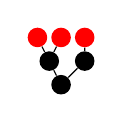
\begin{tikzpicture}[scale=.2]
\node[circle, scale=0.75, fill] (tid0) at (2.25,0){};
\node[circle, scale=0.75, fill] (tid1) at (1.5,1.5){};
\node[circle, scale=0.75, fill, red] (tid3) at (0.75,3){};
\node[circle, scale=0.75, fill, red] (tid4) at (2.25,3){};
\draw[](tid1) -- (tid3);
\draw[](tid1) -- (tid4);
\node[circle, scale=0.75, fill] (tid2) at (3.75,1.5){};
\node[circle, scale=0.75, fill, red] (tid5) at (3.75,3){};
\draw[](tid2) -- (tid5);
\draw[](tid0) -- (tid1);
\draw[](tid0) -- (tid2);

\end{tikzpicture}
\nodepart{two}
\footnotesize{4.05556}
\nodepart{three}
\footnotesize{$67\:33$}
};
\node[draw opacity=0, fill opacity=0, anchor=south west] (dummyL) at (-15, -60){};
\node[draw=black, rectangle split, anchor=south west, rectangle split parts=3] (sn0x8ef6a0) at ([xshift=2cm]dummyL){
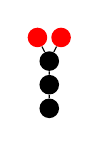
\begin{tikzpicture}[scale=.2]
\node[circle, scale=0.75, fill] (tid0) at (1.5,0){};
\node[circle, scale=0.75, fill] (tid1) at (1.5,1.5){};
\node[circle, scale=0.75, fill] (tid2) at (1.5,3){};
\node[circle, scale=0.75, fill, red] (tid3) at (0.75,4.5){};
\node[circle, scale=0.75, fill, red] (tid4) at (2.25,4.5){};
\draw[](tid2) -- (tid3);
\draw[](tid2) -- (tid4);
\draw[](tid1) -- (tid2);
\draw[](tid0) -- (tid1);

\end{tikzpicture}
\nodepart{two}
\footnotesize{4.5}
\nodepart{three}
\footnotesize{$1$}
};
\node[draw opacity=0, fill opacity=0, anchor=south west] (dummyL) at (-15, -60){};
\node[draw=black, rectangle split, anchor=south west, rectangle split parts=3] (sn0x8ef770) at ([xshift=2cm]sn0x8ef6a0.south east){
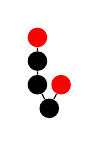
\begin{tikzpicture}[scale=.2]
\node[circle, scale=0.75, fill] (tid0) at (1.5,0){};
\node[circle, scale=0.75, fill] (tid1) at (0.75,1.5){};
\node[circle, scale=0.75, fill] (tid3) at (0.75,3){};
\node[circle, scale=0.75, fill, red] (tid4) at (0.75,4.5){};
\draw[](tid3) -- (tid4);
\draw[](tid1) -- (tid3);
\node[circle, scale=0.75, fill, red] (tid2) at (2.25,1.5){};
\draw[](tid0) -- (tid1);
\draw[](tid0) -- (tid2);

\end{tikzpicture}
\nodepart{two}
\footnotesize{4.125}
\nodepart{three}
\footnotesize{$50\:50$}
};
\node[draw opacity=0, fill opacity=0, anchor=south west] (dummyL) at (-15, -60){};
\node[draw=black, rectangle split, anchor=south west, rectangle split parts=3] (sn0x8f07c0) at ([xshift=2cm]sn0x8ef770.south east){
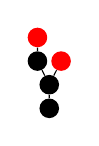
\begin{tikzpicture}[scale=.2]
\node[circle, scale=0.75, fill] (tid0) at (1.5,0){};
\node[circle, scale=0.75, fill] (tid1) at (1.5,1.5){};
\node[circle, scale=0.75, fill] (tid2) at (0.75,3){};
\node[circle, scale=0.75, fill, red] (tid4) at (0.75,4.5){};
\draw[](tid2) -- (tid4);
\node[circle, scale=0.75, fill, red] (tid3) at (2.25,3){};
\draw[](tid1) -- (tid2);
\draw[](tid1) -- (tid3);
\draw[](tid0) -- (tid1);

\end{tikzpicture}
\nodepart{two}
\footnotesize{4.25}
\nodepart{three}
\footnotesize{$50\:50$}
};
\node[draw opacity=0, fill opacity=0, anchor=south west] (dummyL) at (-15, -60){};
\node[draw=black, rectangle split, anchor=south west, rectangle split parts=3] (sn0x8f0950) at ([xshift=2cm]sn0x8f07c0.south east){
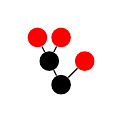
\begin{tikzpicture}[scale=.2]
\node[circle, scale=0.75, fill] (tid0) at (2.25,0){};
\node[circle, scale=0.75, fill] (tid1) at (1.5,1.5){};
\node[circle, scale=0.75, fill, red] (tid3) at (0.75,3){};
\node[circle, scale=0.75, fill, red] (tid4) at (2.25,3){};
\draw[](tid1) -- (tid3);
\draw[](tid1) -- (tid4);
\node[circle, scale=0.75, fill, red] (tid2) at (3.75,1.5){};
\draw[](tid0) -- (tid1);
\draw[](tid0) -- (tid2);

\end{tikzpicture}
\nodepart{two}
\footnotesize{3.66667}
\nodepart{three}
\footnotesize{$33\:67$}
};
\node[draw opacity=0, fill opacity=0, anchor=south west] (dummyL) at (-15, -60){};
\node[draw=black, rectangle split, anchor=south west, rectangle split parts=3] (sn0x8f2260) at ([xshift=2cm]sn0x8f0950.south east){
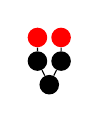
\begin{tikzpicture}[scale=.2]
\node[circle, scale=0.75, fill] (tid0) at (1.5,0){};
\node[circle, scale=0.75, fill] (tid1) at (0.75,1.5){};
\node[circle, scale=0.75, fill, red] (tid3) at (0.75,3){};
\draw[](tid1) -- (tid3);
\node[circle, scale=0.75, fill] (tid2) at (2.25,1.5){};
\node[circle, scale=0.75, fill, red] (tid4) at (2.25,3){};
\draw[](tid2) -- (tid4);
\draw[](tid0) -- (tid1);
\draw[](tid0) -- (tid2);

\end{tikzpicture}
\nodepart{two}
\footnotesize{3.75}
\nodepart{three}
\footnotesize{$1$}
};
\node[draw opacity=0, fill opacity=0, anchor=south west] (dummyL) at (-9, -75){};
\node[draw=black, rectangle split, anchor=south west, rectangle split parts=3] (sn0x8efa00) at ([xshift=2cm]dummyL){
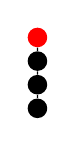
\begin{tikzpicture}[scale=.2]
\node[circle, scale=0.75, fill] (tid0) at (0.75,0){};
\node[circle, scale=0.75, fill] (tid1) at (0.75,1.5){};
\node[circle, scale=0.75, fill] (tid2) at (0.75,3){};
\node[circle, scale=0.75, fill, red] (tid3) at (0.75,4.5){};
\draw[](tid2) -- (tid3);
\draw[](tid1) -- (tid2);
\draw[](tid0) -- (tid1);

\end{tikzpicture}
\nodepart{two}
\footnotesize{4}
\nodepart{three}
\footnotesize{$1$}
};
\node[draw opacity=0, fill opacity=0, anchor=south west] (dummyL) at (-9, -75){};
\node[draw=black, rectangle split, anchor=south west, rectangle split parts=3] (sn0x8efe90) at ([xshift=2cm]sn0x8efa00.south east){
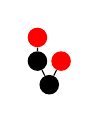
\begin{tikzpicture}[scale=.2]
\node[circle, scale=0.75, fill] (tid0) at (1.5,0){};
\node[circle, scale=0.75, fill] (tid1) at (0.75,1.5){};
\node[circle, scale=0.75, fill, red] (tid3) at (0.75,3){};
\draw[](tid1) -- (tid3);
\node[circle, scale=0.75, fill, red] (tid2) at (2.25,1.5){};
\draw[](tid0) -- (tid1);
\draw[](tid0) -- (tid2);

\end{tikzpicture}
\nodepart{two}
\footnotesize{3.25}
\nodepart{three}
\footnotesize{$50\:50$}
};
\node[draw opacity=0, fill opacity=0, anchor=south west] (dummyL) at (-9, -75){};
\node[draw=black, rectangle split, anchor=south west, rectangle split parts=3] (sn0x8f1240) at ([xshift=2cm]sn0x8efe90.south east){
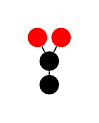
\begin{tikzpicture}[scale=.2]
\node[circle, scale=0.75, fill] (tid0) at (1.5,0){};
\node[circle, scale=0.75, fill] (tid1) at (1.5,1.5){};
\node[circle, scale=0.75, fill, red] (tid2) at (0.75,3){};
\node[circle, scale=0.75, fill, red] (tid3) at (2.25,3){};
\draw[](tid1) -- (tid2);
\draw[](tid1) -- (tid3);
\draw[](tid0) -- (tid1);

\end{tikzpicture}
\nodepart{two}
\footnotesize{3.5}
\nodepart{three}
\footnotesize{$1$}
};
\node[draw opacity=0, fill opacity=0, anchor=south west] (dummyL) at (-6, -90){};
\node[draw=black, rectangle split, anchor=south west, rectangle split parts=3] (sn0x8efb50) at ([xshift=2cm]dummyL){
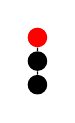
\begin{tikzpicture}[scale=.2]
\node[circle, scale=0.75, fill] (tid0) at (0.75,0){};
\node[circle, scale=0.75, fill] (tid1) at (0.75,1.5){};
\node[circle, scale=0.75, fill, red] (tid2) at (0.75,3){};
\draw[](tid1) -- (tid2);
\draw[](tid0) -- (tid1);

\end{tikzpicture}
\nodepart{two}
\footnotesize{3}
\nodepart{three}
\footnotesize{$1$}
};
\node[draw opacity=0, fill opacity=0, anchor=south west] (dummyL) at (-6, -90){};
\node[draw=black, rectangle split, anchor=south west, rectangle split parts=3] (sn0x8f02e0) at ([xshift=2cm]sn0x8efb50.south east){

\begin{tikzpicture}[scale=.2]
\node[circle, scale=0.75, fill] (tid0) at (1.5,0){};
\node[circle, scale=0.75, fill, red] (tid1) at (0.75,1.5){};
\node[circle, scale=0.75, fill, red] (tid2) at (2.25,1.5){};
\draw[](tid0) -- (tid1);
\draw[](tid0) -- (tid2);

\end{tikzpicture}
\nodepart{two}
\footnotesize{2.5}
\nodepart{three}
\footnotesize{$1$}
};
\draw (sn0x8eb820.south) -- (sn0x8ee960.north);
\draw (sn0x8eb820.south) -- (sn0x8ee260.north);
\draw (sn0x8ee960.south) -- (sn0x8ef400.north);
\draw (sn0x8ee960.south) -- (sn0x8ef140.north);
\draw (sn0x8ee260.south) -- (sn0x8f19a0.north);
\draw (sn0x8ee260.south) -- (sn0x8ef140.north);
\draw (sn0x8ee260.south) -- (sn0x8f1400.north);
\draw (sn0x8ef400.south) -- (sn0x8ef6a0.north);
\draw (sn0x8ef400.south) -- (sn0x8ef770.north);
\draw (sn0x8ef140.south) -- (sn0x8f07c0.north);
\draw (sn0x8ef140.south) -- (sn0x8ef770.north);
\draw (sn0x8ef140.south) -- (sn0x8f0950.north);
\draw (sn0x8f19a0.south) -- (sn0x8ef770.north);
\draw (sn0x8f19a0.south) -- (sn0x8f2260.north);
\draw (sn0x8f1400.south) -- (sn0x8f2260.north);
\draw (sn0x8f1400.south) -- (sn0x8f0950.north);
\draw (sn0x8ef6a0.south) -- (sn0x8efa00.north);
\draw (sn0x8ef770.south) -- (sn0x8efa00.north);
\draw (sn0x8ef770.south) -- (sn0x8efe90.north);
\draw (sn0x8f07c0.south) -- (sn0x8efa00.north);
\draw (sn0x8f07c0.south) -- (sn0x8f1240.north);
\draw (sn0x8f0950.south) -- (sn0x8f1240.north);
\draw (sn0x8f0950.south) -- (sn0x8efe90.north);
\draw (sn0x8f2260.south) -- (sn0x8efe90.north);
\draw (sn0x8efa00.south) -- (sn0x8efb50.north);
\draw (sn0x8efe90.south) -- (sn0x8efb50.north);
\draw (sn0x8efe90.south) -- (sn0x8f02e0.north);
\draw (sn0x8f1240.south) -- (sn0x8efb50.north);
\end{tikzpicture}

%%% Local Variables:
%%% TeX-master: "thesis/thesis.tex"
%%% End: 

\begin{tikzpicture}[scale=.2, anchor=west]
\node[draw opacity=0, fill opacity=0, anchor=south west] (dummyL) at (-3, -15){};
\node[draw=black, rectangle split, anchor=south west, rectangle split parts=3] (sn0x8eb8e0) at ([xshift=2cm]dummyL){
\begin{tikzpicture}[scale=.2]
\node[circle, scale=0.75, fill] (tid0) at (3,0){};
\node[circle, scale=0.75, fill] (tid1) at (2.25,1.5){};
\node[circle, scale=0.75, fill] (tid3) at (1.5,3){};
\node[circle, scale=0.75, fill, red] (tid6) at (0.75,4.5){};
\node[circle, scale=0.75, fill, red] (tid7) at (2.25,4.5){};
\draw[](tid3) -- (tid6);
\draw[](tid3) -- (tid7);
\node[circle, scale=0.75, fill, red] (tid4) at (3.75,3){};
\draw[](tid1) -- (tid3);
\draw[](tid1) -- (tid4);
\node[circle, scale=0.75, fill] (tid2) at (5.25,1.5){};
\node[circle, scale=0.75, fill] (tid5) at (5.25,3){};
\draw[](tid2) -- (tid5);
\draw[](tid0) -- (tid1);
\draw[](tid0) -- (tid2);

\end{tikzpicture}
\nodepart{two}
\footnotesize{5.01543}
\nodepart{three}
\footnotesize{$33\:67$}
};
\node[draw opacity=0, fill opacity=0, anchor=south west] (dummyL) at (-6, -30){};
\node[draw=black, rectangle split, anchor=south west, rectangle split parts=3] (sn0x8f2890) at ([xshift=2cm]dummyL){
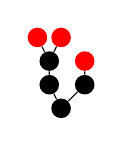
\begin{tikzpicture}[scale=.2]
\node[circle, scale=0.75, fill] (tid0) at (2.25,0){};
\node[circle, scale=0.75, fill] (tid1) at (1.5,1.5){};
\node[circle, scale=0.75, fill] (tid3) at (1.5,3){};
\node[circle, scale=0.75, fill, red] (tid5) at (0.75,4.5){};
\node[circle, scale=0.75, fill, red] (tid6) at (2.25,4.5){};
\draw[](tid3) -- (tid5);
\draw[](tid3) -- (tid6);
\draw[](tid1) -- (tid3);
\node[circle, scale=0.75, fill] (tid2) at (3.75,1.5){};
\node[circle, scale=0.75, fill, red] (tid4) at (3.75,3){};
\draw[](tid2) -- (tid4);
\draw[](tid0) -- (tid1);
\draw[](tid0) -- (tid2);

\end{tikzpicture}
\nodepart{two}
\footnotesize{4.81944}
\nodepart{three}
\footnotesize{$33\:67$}
};
\node[draw opacity=0, fill opacity=0, anchor=south west] (dummyL) at (-6, -30){};
\node[draw=black, rectangle split, anchor=south west, rectangle split parts=3] (sn0x8ee260) at ([xshift=2cm]sn0x8f2890.south east){
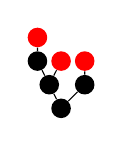
\begin{tikzpicture}[scale=.2]
\node[circle, scale=0.75, fill] (tid0) at (2.25,0){};
\node[circle, scale=0.75, fill] (tid1) at (1.5,1.5){};
\node[circle, scale=0.75, fill] (tid3) at (0.75,3){};
\node[circle, scale=0.75, fill, red] (tid6) at (0.75,4.5){};
\draw[](tid3) -- (tid6);
\node[circle, scale=0.75, fill, red] (tid4) at (2.25,3){};
\draw[](tid1) -- (tid3);
\draw[](tid1) -- (tid4);
\node[circle, scale=0.75, fill] (tid2) at (3.75,1.5){};
\node[circle, scale=0.75, fill, red] (tid5) at (3.75,3){};
\draw[](tid2) -- (tid5);
\draw[](tid0) -- (tid1);
\draw[](tid0) -- (tid2);

\end{tikzpicture}
\nodepart{two}
\footnotesize{4.61343}
\nodepart{three}
\footnotesize{$33\:33\:33$}
};
\node[draw opacity=0, fill opacity=0, anchor=south west] (dummyL) at (-12, -45){};
\node[draw=black, rectangle split, anchor=south west, rectangle split parts=3] (sn0x8ef400) at ([xshift=2cm]dummyL){
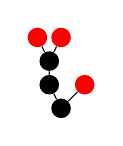
\begin{tikzpicture}[scale=.2]
\node[circle, scale=0.75, fill] (tid0) at (2.25,0){};
\node[circle, scale=0.75, fill] (tid1) at (1.5,1.5){};
\node[circle, scale=0.75, fill] (tid3) at (1.5,3){};
\node[circle, scale=0.75, fill, red] (tid4) at (0.75,4.5){};
\node[circle, scale=0.75, fill, red] (tid5) at (2.25,4.5){};
\draw[](tid3) -- (tid4);
\draw[](tid3) -- (tid5);
\draw[](tid1) -- (tid3);
\node[circle, scale=0.75, fill, red] (tid2) at (3.75,1.5){};
\draw[](tid0) -- (tid1);
\draw[](tid0) -- (tid2);

\end{tikzpicture}
\nodepart{two}
\footnotesize{4.58333}
\nodepart{three}
\footnotesize{$33\:67$}
};
\node[draw opacity=0, fill opacity=0, anchor=south west] (dummyL) at (-12, -45){};
\node[draw=black, rectangle split, anchor=south west, rectangle split parts=3] (sn0x8f19a0) at ([xshift=2cm]sn0x8ef400.south east){
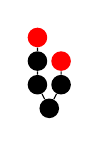
\begin{tikzpicture}[scale=.2]
\node[circle, scale=0.75, fill] (tid0) at (1.5,0){};
\node[circle, scale=0.75, fill] (tid1) at (0.75,1.5){};
\node[circle, scale=0.75, fill] (tid3) at (0.75,3){};
\node[circle, scale=0.75, fill, red] (tid5) at (0.75,4.5){};
\draw[](tid3) -- (tid5);
\draw[](tid1) -- (tid3);
\node[circle, scale=0.75, fill] (tid2) at (2.25,1.5){};
\node[circle, scale=0.75, fill, red] (tid4) at (2.25,3){};
\draw[](tid2) -- (tid4);
\draw[](tid0) -- (tid1);
\draw[](tid0) -- (tid2);

\end{tikzpicture}
\nodepart{two}
\footnotesize{4.4375}
\nodepart{three}
\footnotesize{$50\:50$}
};
\node[draw opacity=0, fill opacity=0, anchor=south west] (dummyL) at (-12, -45){};
\node[draw=black, rectangle split, anchor=south west, rectangle split parts=3] (sn0x8ef140) at ([xshift=2cm]sn0x8f19a0.south east){
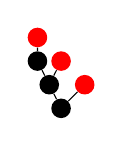
\begin{tikzpicture}[scale=.2]
\node[circle, scale=0.75, fill] (tid0) at (2.25,0){};
\node[circle, scale=0.75, fill] (tid1) at (1.5,1.5){};
\node[circle, scale=0.75, fill] (tid3) at (0.75,3){};
\node[circle, scale=0.75, fill, red] (tid5) at (0.75,4.5){};
\draw[](tid3) -- (tid5);
\node[circle, scale=0.75, fill, red] (tid4) at (2.25,3){};
\draw[](tid1) -- (tid3);
\draw[](tid1) -- (tid4);
\node[circle, scale=0.75, fill, red] (tid2) at (3.75,1.5){};
\draw[](tid0) -- (tid1);
\draw[](tid0) -- (tid2);

\end{tikzpicture}
\nodepart{two}
\footnotesize{4.34722}
\nodepart{three}
\footnotesize{$33\:33\:33$}
};
\node[draw opacity=0, fill opacity=0, anchor=south west] (dummyL) at (-12, -45){};
\node[draw=black, rectangle split, anchor=south west, rectangle split parts=3] (sn0x8f1400) at ([xshift=2cm]sn0x8ef140.south east){
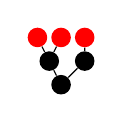
\begin{tikzpicture}[scale=.2]
\node[circle, scale=0.75, fill] (tid0) at (2.25,0){};
\node[circle, scale=0.75, fill] (tid1) at (1.5,1.5){};
\node[circle, scale=0.75, fill, red] (tid3) at (0.75,3){};
\node[circle, scale=0.75, fill, red] (tid4) at (2.25,3){};
\draw[](tid1) -- (tid3);
\draw[](tid1) -- (tid4);
\node[circle, scale=0.75, fill] (tid2) at (3.75,1.5){};
\node[circle, scale=0.75, fill, red] (tid5) at (3.75,3){};
\draw[](tid2) -- (tid5);
\draw[](tid0) -- (tid1);
\draw[](tid0) -- (tid2);

\end{tikzpicture}
\nodepart{two}
\footnotesize{4.05556}
\nodepart{three}
\footnotesize{$67\:33$}
};
\node[draw opacity=0, fill opacity=0, anchor=south west] (dummyL) at (-15, -60){};
\node[draw=black, rectangle split, anchor=south west, rectangle split parts=3] (sn0x8ef6a0) at ([xshift=2cm]dummyL){
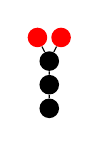
\begin{tikzpicture}[scale=.2]
\node[circle, scale=0.75, fill] (tid0) at (1.5,0){};
\node[circle, scale=0.75, fill] (tid1) at (1.5,1.5){};
\node[circle, scale=0.75, fill] (tid2) at (1.5,3){};
\node[circle, scale=0.75, fill, red] (tid3) at (0.75,4.5){};
\node[circle, scale=0.75, fill, red] (tid4) at (2.25,4.5){};
\draw[](tid2) -- (tid3);
\draw[](tid2) -- (tid4);
\draw[](tid1) -- (tid2);
\draw[](tid0) -- (tid1);

\end{tikzpicture}
\nodepart{two}
\footnotesize{4.5}
\nodepart{three}
\footnotesize{$1$}
};
\node[draw opacity=0, fill opacity=0, anchor=south west] (dummyL) at (-15, -60){};
\node[draw=black, rectangle split, anchor=south west, rectangle split parts=3] (sn0x8ef770) at ([xshift=2cm]sn0x8ef6a0.south east){
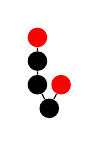
\begin{tikzpicture}[scale=.2]
\node[circle, scale=0.75, fill] (tid0) at (1.5,0){};
\node[circle, scale=0.75, fill] (tid1) at (0.75,1.5){};
\node[circle, scale=0.75, fill] (tid3) at (0.75,3){};
\node[circle, scale=0.75, fill, red] (tid4) at (0.75,4.5){};
\draw[](tid3) -- (tid4);
\draw[](tid1) -- (tid3);
\node[circle, scale=0.75, fill, red] (tid2) at (2.25,1.5){};
\draw[](tid0) -- (tid1);
\draw[](tid0) -- (tid2);

\end{tikzpicture}
\nodepart{two}
\footnotesize{4.125}
\nodepart{three}
\footnotesize{$50\:50$}
};
\node[draw opacity=0, fill opacity=0, anchor=south west] (dummyL) at (-15, -60){};
\node[draw=black, rectangle split, anchor=south west, rectangle split parts=3] (sn0x8f2260) at ([xshift=2cm]sn0x8ef770.south east){
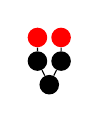
\begin{tikzpicture}[scale=.2]
\node[circle, scale=0.75, fill] (tid0) at (1.5,0){};
\node[circle, scale=0.75, fill] (tid1) at (0.75,1.5){};
\node[circle, scale=0.75, fill, red] (tid3) at (0.75,3){};
\draw[](tid1) -- (tid3);
\node[circle, scale=0.75, fill] (tid2) at (2.25,1.5){};
\node[circle, scale=0.75, fill, red] (tid4) at (2.25,3){};
\draw[](tid2) -- (tid4);
\draw[](tid0) -- (tid1);
\draw[](tid0) -- (tid2);

\end{tikzpicture}
\nodepart{two}
\footnotesize{3.75}
\nodepart{three}
\footnotesize{$1$}
};
\node[draw opacity=0, fill opacity=0, anchor=south west] (dummyL) at (-15, -60){};
\node[draw=black, rectangle split, anchor=south west, rectangle split parts=3] (sn0x8f07c0) at ([xshift=2cm]sn0x8f2260.south east){
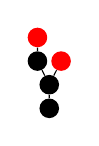
\begin{tikzpicture}[scale=.2]
\node[circle, scale=0.75, fill] (tid0) at (1.5,0){};
\node[circle, scale=0.75, fill] (tid1) at (1.5,1.5){};
\node[circle, scale=0.75, fill] (tid2) at (0.75,3){};
\node[circle, scale=0.75, fill, red] (tid4) at (0.75,4.5){};
\draw[](tid2) -- (tid4);
\node[circle, scale=0.75, fill, red] (tid3) at (2.25,3){};
\draw[](tid1) -- (tid2);
\draw[](tid1) -- (tid3);
\draw[](tid0) -- (tid1);

\end{tikzpicture}
\nodepart{two}
\footnotesize{4.25}
\nodepart{three}
\footnotesize{$50\:50$}
};
\node[draw opacity=0, fill opacity=0, anchor=south west] (dummyL) at (-15, -60){};
\node[draw=black, rectangle split, anchor=south west, rectangle split parts=3] (sn0x8f0950) at ([xshift=2cm]sn0x8f07c0.south east){
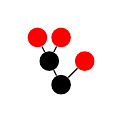
\begin{tikzpicture}[scale=.2]
\node[circle, scale=0.75, fill] (tid0) at (2.25,0){};
\node[circle, scale=0.75, fill] (tid1) at (1.5,1.5){};
\node[circle, scale=0.75, fill, red] (tid3) at (0.75,3){};
\node[circle, scale=0.75, fill, red] (tid4) at (2.25,3){};
\draw[](tid1) -- (tid3);
\draw[](tid1) -- (tid4);
\node[circle, scale=0.75, fill, red] (tid2) at (3.75,1.5){};
\draw[](tid0) -- (tid1);
\draw[](tid0) -- (tid2);

\end{tikzpicture}
\nodepart{two}
\footnotesize{3.66667}
\nodepart{three}
\footnotesize{$33\:67$}
};
\node[draw opacity=0, fill opacity=0, anchor=south west] (dummyL) at (-9, -75){};
\node[draw=black, rectangle split, anchor=south west, rectangle split parts=3] (sn0x8efa00) at ([xshift=2cm]dummyL){
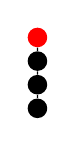
\begin{tikzpicture}[scale=.2]
\node[circle, scale=0.75, fill] (tid0) at (0.75,0){};
\node[circle, scale=0.75, fill] (tid1) at (0.75,1.5){};
\node[circle, scale=0.75, fill] (tid2) at (0.75,3){};
\node[circle, scale=0.75, fill, red] (tid3) at (0.75,4.5){};
\draw[](tid2) -- (tid3);
\draw[](tid1) -- (tid2);
\draw[](tid0) -- (tid1);

\end{tikzpicture}
\nodepart{two}
\footnotesize{4}
\nodepart{three}
\footnotesize{$1$}
};
\node[draw opacity=0, fill opacity=0, anchor=south west] (dummyL) at (-9, -75){};
\node[draw=black, rectangle split, anchor=south west, rectangle split parts=3] (sn0x8efe90) at ([xshift=2cm]sn0x8efa00.south east){
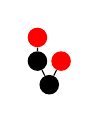
\begin{tikzpicture}[scale=.2]
\node[circle, scale=0.75, fill] (tid0) at (1.5,0){};
\node[circle, scale=0.75, fill] (tid1) at (0.75,1.5){};
\node[circle, scale=0.75, fill, red] (tid3) at (0.75,3){};
\draw[](tid1) -- (tid3);
\node[circle, scale=0.75, fill, red] (tid2) at (2.25,1.5){};
\draw[](tid0) -- (tid1);
\draw[](tid0) -- (tid2);

\end{tikzpicture}
\nodepart{two}
\footnotesize{3.25}
\nodepart{three}
\footnotesize{$50\:50$}
};
\node[draw opacity=0, fill opacity=0, anchor=south west] (dummyL) at (-9, -75){};
\node[draw=black, rectangle split, anchor=south west, rectangle split parts=3] (sn0x8f1240) at ([xshift=2cm]sn0x8efe90.south east){
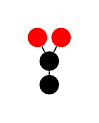
\begin{tikzpicture}[scale=.2]
\node[circle, scale=0.75, fill] (tid0) at (1.5,0){};
\node[circle, scale=0.75, fill] (tid1) at (1.5,1.5){};
\node[circle, scale=0.75, fill, red] (tid2) at (0.75,3){};
\node[circle, scale=0.75, fill, red] (tid3) at (2.25,3){};
\draw[](tid1) -- (tid2);
\draw[](tid1) -- (tid3);
\draw[](tid0) -- (tid1);

\end{tikzpicture}
\nodepart{two}
\footnotesize{3.5}
\nodepart{three}
\footnotesize{$1$}
};
\node[draw opacity=0, fill opacity=0, anchor=south west] (dummyL) at (-6, -90){};
\node[draw=black, rectangle split, anchor=south west, rectangle split parts=3] (sn0x8efb50) at ([xshift=2cm]dummyL){
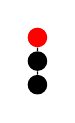
\begin{tikzpicture}[scale=.2]
\node[circle, scale=0.75, fill] (tid0) at (0.75,0){};
\node[circle, scale=0.75, fill] (tid1) at (0.75,1.5){};
\node[circle, scale=0.75, fill, red] (tid2) at (0.75,3){};
\draw[](tid1) -- (tid2);
\draw[](tid0) -- (tid1);

\end{tikzpicture}
\nodepart{two}
\footnotesize{3}
\nodepart{three}
\footnotesize{$1$}
};
\node[draw opacity=0, fill opacity=0, anchor=south west] (dummyL) at (-6, -90){};
\node[draw=black, rectangle split, anchor=south west, rectangle split parts=3] (sn0x8f02e0) at ([xshift=2cm]sn0x8efb50.south east){

\begin{tikzpicture}[scale=.2]
\node[circle, scale=0.75, fill] (tid0) at (1.5,0){};
\node[circle, scale=0.75, fill, red] (tid1) at (0.75,1.5){};
\node[circle, scale=0.75, fill, red] (tid2) at (2.25,1.5){};
\draw[](tid0) -- (tid1);
\draw[](tid0) -- (tid2);

\end{tikzpicture}
\nodepart{two}
\footnotesize{2.5}
\nodepart{three}
\footnotesize{$1$}
};
\draw (sn0x8eb8e0.south) -- (sn0x8f2890.north);
\draw (sn0x8eb8e0.south) -- (sn0x8ee260.north);
\draw (sn0x8f2890.south) -- (sn0x8ef400.north);
\draw (sn0x8f2890.south) -- (sn0x8f19a0.north);
\draw (sn0x8ee260.south) -- (sn0x8f19a0.north);
\draw (sn0x8ee260.south) -- (sn0x8ef140.north);
\draw (sn0x8ee260.south) -- (sn0x8f1400.north);
\draw (sn0x8ef400.south) -- (sn0x8ef6a0.north);
\draw (sn0x8ef400.south) -- (sn0x8ef770.north);
\draw (sn0x8f19a0.south) -- (sn0x8ef770.north);
\draw (sn0x8f19a0.south) -- (sn0x8f2260.north);
\draw (sn0x8ef140.south) -- (sn0x8f07c0.north);
\draw (sn0x8ef140.south) -- (sn0x8ef770.north);
\draw (sn0x8ef140.south) -- (sn0x8f0950.north);
\draw (sn0x8f1400.south) -- (sn0x8f2260.north);
\draw (sn0x8f1400.south) -- (sn0x8f0950.north);
\draw (sn0x8ef6a0.south) -- (sn0x8efa00.north);
\draw (sn0x8ef770.south) -- (sn0x8efa00.north);
\draw (sn0x8ef770.south) -- (sn0x8efe90.north);
\draw (sn0x8f2260.south) -- (sn0x8efe90.north);
\draw (sn0x8f07c0.south) -- (sn0x8efa00.north);
\draw (sn0x8f07c0.south) -- (sn0x8f1240.north);
\draw (sn0x8f0950.south) -- (sn0x8f1240.north);
\draw (sn0x8f0950.south) -- (sn0x8efe90.north);
\draw (sn0x8efa00.south) -- (sn0x8efb50.north);
\draw (sn0x8efe90.south) -- (sn0x8efb50.north);
\draw (sn0x8efe90.south) -- (sn0x8f02e0.north);
\draw (sn0x8f1240.south) -- (sn0x8efb50.north);
\end{tikzpicture}

%%% Local Variables:
%%% TeX-master: "thesis/thesis.tex"
%%% End: 

